\documentclass[a4paper,reqno]{amsart}
\usepackage{amssymb}
\usepackage{amsmath}
\usepackage{tikz}

\begin{document}

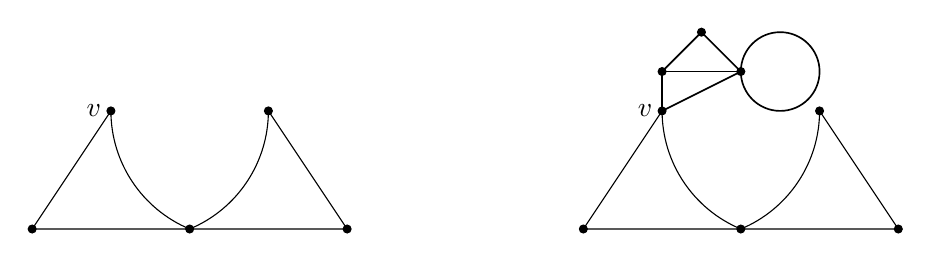
\begin{tikzpicture}
    \draw[fill] (0,0) circle(0.05);
    \draw[fill] (2,0) circle(0.05);
    \draw[fill] (1,1.5) circle(0.05) node[left]{$v$};
    \draw[fill] (4,0) circle(0.05);
    \draw[fill] (3,1.5) circle(0.05);
    \draw (1,1.5)--(0,0)--(2,0);
    \draw (2,0)--(4,0)--(3,1.5);
    \draw (1,1.5) arc(180:247.38:1.625);
    \draw (3,1.5) arc(0:-67.38:1.625);
    \begin{scope}[shift={(7,0)}]
      \draw[fill] (0,0) circle(0.05);
      \draw[fill] (2,0) circle(0.05);
      \draw[fill] (1,1.5) circle(0.05) node[left]{$v$};
      \draw[fill] (4,0) circle(0.05);
      \draw[fill] (3,1.5) circle(0.05);
      \draw (1,1.5)--(0,0)--(2,0);
      \draw (2,0)--(4,0)--(3,1.5);
      \draw (1,1.5) arc(180:247.38:1.625);
      \draw (3,1.5) arc(0:-67.38:1.625);
      \draw[fill] (2,2) circle(0.05);
      \draw[fill] (1.5,2.5) circle(0.05);
      \draw[fill] (1,2) circle(0.05);
      \draw[semithick] (1,1.5)--(2,2);
      \draw[semithick] (1,1.5)--(1,2);
      \draw[semithick] (1,2)--(2,2);
      \draw[semithick] (1.5,2.5)--(2,2);
      \draw[semithick] (1,2)--(1.5,2.5);
      \draw[semithick] (2.5,2) circle(0.5);
    \end{scope}
  \end{tikzpicture}

\end{document}